% Name: Turing machine
% Description: A simple Turing machine state diagram.
% Tags: turing machine, computability

\usetikzlibrary{automata, positioning}

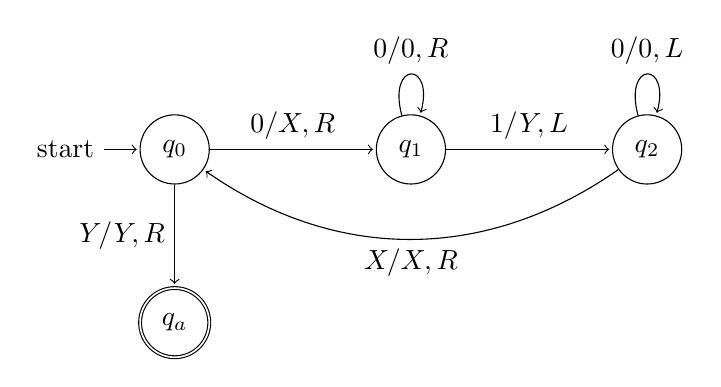
\begin{tikzpicture}[shorten >=1pt, node distance=3cm, on grid, auto]
  \node[state, initial] (q0) {$q_0$};
  \node[state] (q1) [right=of q0] {$q_1$};
  \node[state] (q2) [right=of q1] {$q_2$};
  \node[state, accepting] (qa) [below=2.2cm of q0] {$q_a$};

  \path[->]
    (q0) edge node{$0/X, R$} (q1)
    (q1) edge[loop above] node{$0/0, R$} ()
         edge node{$1/Y, L$} (q2)
    (q2) edge[loop above] node{$0/0, L$} ()
         edge[bend left=35] node{$X/X, R$} (q0)
    (q0) edge node[left]{$Y/Y, R$} (qa);
\end{tikzpicture}
